\chapter{Adaption of example applications}
\label{ch:adaption}
In this chapter, to show the feasibility of the approach, two open-source e-mail clients adapted to support run-time state migration based on the developed approach as part of the thesis.

As a developer who wants to implement the enabling run-time state migration, we used the developed approach, middleware, libraries, deriving interfaces, and adaptability to existing same-purpose applications. 

\section{Application State Models}
After analyzing states of Mailspring and K-9 Mail applications and their source code (Table \ref{tab:states_of_email_applications}), we decided to model \textit{search} and \textit{sending-email} states. We have developed two common Application State Models in Chapter \ref{ch:language} for these two applications which are Listing \ref{lis:search-schema} and \ref{lis:sending-email-schema}. 



\section{Example Applications}
These applications are for different platforms, and their source code is freely accessible to allow the integration of libraries. 
Suggestions for e-mail clients to be adapted are K-9 Mail for Android and Mailspring for desktop operating systems. They are interactive applications for end-users and have sufficient complexity (e.g., applications do not have only one single state).
K-9 Mail Android application is developed in Java; therefore, it requires the Android library, which we developed for run-time state migration. Moreover, Mailspring is developed using Electron and TypeScript for desktop operating systems, and it needs the JavaScript library for run-time state migration.

\subsection{Mailspring}
Mailspring is an open-source e-mail client application\footnote{\url{https://getmailspring.com/}}. The source code of this application is available on GitHub\footnote{\url{https://github.com/Foundry376/Mailspring}}. This application can be installed on desktop operating systems like macOS, Linux, and Windows.
\subsubsection{Architecture}
Because Mailspring is written in TypeScript (which is a superset of JavaScript) and has been built on top of Electron, its main script which specified in \lstinline[basicstyle=\ttfamily]{package.json}, is referred to as the main process. The main process's script can display a UI by generating web pages. Only one main process is involved in an Electron application. Also, Electron has another type of process, which is the renderer process, and each web page runs in its own renderer process. Electron provides a special API for communication of main process and renderer processes \cite{electron}. Furthermore, Mailspring's UI is developed in ReactJS, which is a JavaScript UI library. Each part of the UI is a ReactJS component.

\subsubsection{Adaptions}
The run-time state migration JavaScript library and Application State Models interfaces are integrated into the main process's script. On the other hand, all UI adaptions are in ReactJS components. Adaptions are added to the fork of this project, hosted on GitHub\footnote{\url{https://github.com/asml-lang/mailspring}}. 

Following is a brief description of the main implementation parts in Mailspring.

\paragraph{Library Usage}
The main process's script of Mailspring is implemented in \lstinline[basicstyle=\ttfamily]{application.ts} which is in \lstinline[basicstyle=\ttfamily]{app/src/browser/} directory.
We have imported the JavaScript library of run-time state migration, \textit{search} and \textit{sending-email} Application State Models and their interfaces in this script. Listing \ref{lis:js-import} shows how this import is done.

\FloatBarrier
\begin{code}
\begin{js2}
import RuntimeStateMigration from 'rsm-node';
import sendingEmail from '../models/sending-email.json';
import searchEmail from '../models/search.json';
import { 
    SearchObject,
    Convert as SearchObjectConvert
} from '../models/Search';
import {
    SendingEmailObject,
    Convert as SendingEmailObjectConvert
} from '../models/SendingEmail';
\end{js2}
\caption{Import of JavaScript library of run-time state migration, Application State Models and their interfaces}
\label{lis:js-import}
\end{code}
\FloatBarrier

\paragraph{Application Initialization}
The main process's script has a entry point which is \lstinline[basicstyle=\ttfamily]{start} method. An instance of JavaScript library has been made in this method with some configuration parameters. Also, callback methods which we have implemented in main process's script are bound to the instance of the library as parameters. Furthermore, 
Application State Models are added in this method which \textit{addModel} method. Moreover, \textit{DeviceIntroduction} method is being call here. Listing \ref{lis:js-app-init} shows a snippet that we use to implement the instruction above.

\FloatBarrier
\begin{code}
\begin{js2}
this.rsm = new RuntimeStateMigration(
  { 
    name: 'Mailspring MAC',
    server: {
        url: 'mqtt://130.185.123.111',
        port: 1883
    }
  },
  this.rsmOnStateRequest.bind(this),
  this.rsmOnStateReceive.bind(this),
  this.rsmOnStateMigration.bind(this),
  this.rsmOnDeviceJoin.bind(this),
  this.rsmOnDeviceLeave.bind(this),
);

this.rsm.addModel(sendingEmail);
this.rsm.addModel(searchEmail);
this.rsm.introduce();
\end{js2}
\caption{Application initialization necessary codes}
\label{lis:js-app-init}
\end{code}
\FloatBarrier

\paragraph{Transferring Run-time State}
In case of any changing in inputs of \textit{search} and \textit{compose} views in Mailspring, the current run-time state of them is being stored with \textit{setState} in library, in case of an application request for them. Also, other devices with the same Application State Model should be noticed when this device has a state or not with \textit{setHasState} method. Listing \ref{lis:js-setate} shows how we used this method for \textit{search} state.

\FloatBarrier
\begin{code}
\begin{js2}
const model_name = 'search';

this.rsm.setHasState(model_name, true);

const search: SearchObject = state;
this.rsm.setState(model_name, search);
\end{js2}
\caption{Using the setState and setHasState methods}
\label{lis:js-setate}
\end{code}
\FloatBarrier


As we discussed in Chapter \ref{ch:implementation}, when any device request for run-time state of the source application, the \textit{onStateRequest} callback will be called. Listing \ref{lis:js-request} shows how we have implemented this method in Mailspring. 
  
\FloatBarrier
\begin{code}
\begin{js2}
rsmOnStateRequest(data) {
   this.rsm.sendState(data.model_name, data.device.id);
}
\end{js2}
\caption{Using the onStateRequest method}
\label{lis:js-request}
\end{code}
\FloatBarrier

When a device receive a state the \textit{onStateReceive} callback will be called. In Mailspring we wrote a code in \textit{rsmOnStateReceive} method to find the corresponding window by and send the run-time state to UI with Electron \lstinline[basicstyle=\ttfamily]{ipcRenderer} by \textit{transferToWindow} method. In UI components we implemented a method to adjust the new run-time state. Listing \ref{lis:js-receive} shows a method that adjust the new run-time state of \textit{search} state.

\FloatBarrier
\begin{code}
\begin{js2}

rsmOnStateReceive(data) {
    this.transferToWindow(data.model_name, data.state);
}

// UI Code Example
_onState = (data, wndwKey) => {
    const search: SearchObject = SearchObjectConvert.toSearch(data);
    
    // Mailspring native variable and methods that we have changed
    this._searchQuery = search.query || "";
    this._submit = search.submit || false;
    this.trigger();
};
\end{js2}
\caption{Using the onStateReceive method to adjust new run-time state}
\label{lis:js-receive}
\end{code}
\FloatBarrier

After finishing the migration, the target device should notify the source device about finalizing the run-time state migration with \textit{setMigration} method. In Mailspring we changed the UI to call \textit{setMigration} method when the run-time state adjusted. Listing \ref{lis:js-mg-set} shows this implementation for \textit{search} state.
Also, when the source device receives the migration message and \textit{onStateMigration} callback is being called, its the run-time state should be reset. Listing \ref{lis:js-mg-get} shows how we implement this callback. 

\FloatBarrier
\begin{code}
\begin{js2}
const model_name = 'search';
this.rsm.setMigration(model_name, source_device_id);
\end{js2}
\caption{Notifying source device the migration is complete}
\label{lis:js-mg-set}
\end{code}
\FloatBarrier

\FloatBarrier
\begin{code}
\begin{js2}
rsmOnStateMigration(data) {
    const search: SearchObject = {};
    this.rsm.setState(data.model_name, SearchObject);
    this.rsm.setHasState(data.model_name, false);
}
\end{js2}
\caption{Resetting the run-time state when get a migration message}
\label{lis:js-mg-get}
\end{code}
\FloatBarrier


\subsection{K-9 Mail}
K-9 Mail is an open-source e-mail client application\footnote{\url{https://k9mail.app/}}. The source code of this application is available on GitHub\footnote{\url{https://github.com/k9mail/k-9}}. This application can be installed on Android devices.

\subsubsection{Architecture}
K-9 Mail is written in Java 8. However, the new code base is migrating to Kotlin. The K-9 Mail project consists of different modules. The \textit{k9mail} is the main module that includes code for database interaction, notification, and activities. Another module is the \textit{k9mail-library} which is the back-end code for decoding e-mails and contacting mail providers. 

\subsubsection{Adaptions}
As we worked only on the application, all changes are implemented in \textit{k9mail} module. The run-time state migration Android library has been added to this module as a dependency. The \textit{k9mail} consist of different packages. The integration of run-time state migration is implemented in \textit{ui} package.

Adaptions are added to the fork of this project, hosted on GitHub\footnote{\url{https://github.com/asml-lang/k-9}}. 


\subsection{UI Adaptions}
In this section, we explain all implemented UI adaptions in both applications to achieve a proper behavior of run-time state migration. 

\subsubsection{Notifications}
When a device joins or leaves, other devices which are subscribed to the same Application State Model's topic will be notified by \textit{onDeviceJoin} and \textit{onDeviceLeave} callbacks. Devices that gets this message show a native notification on their application and inform the user about the connectivity status of the device.

\subsubsection{Run-time State Migration Button}
For each view of a state, we developed a floating action button as the main button of run-time state migration. When the user clicks on this button, applications display two other buttons as \textit{Set State} for push method and \textit{Get State} for the pull method. The user can start the migration process by clicking one of these buttons on the current run-time state. Figures \ref{fig:adapt-noti} and \ref{fig:adapt-compose} show run-time state migration button on different views of Mailspring and K-9 Mail. 

\subsubsection{Device List Modal Box}
When the user clicks on the run-time state migration button and clicks on one of the migration methods' buttons, applications show a modal box. This modal box displays the name of the current run-time state, migration method, and the list of the devices available for migration by \textit{getDevices}. The user should select a device from the list and click on the \textit{migrate} button. By clicking on the \textit{migrate} button, If the chosen method is push, the run-time state can be migrated by \textit{sendState} method explained in 7.3.1. Otherwise, for the pull method, the run-time state can be requested by \textit{getStateDevice}. In the end, the modal box gets closed. Figure \ref{fig:adapt-modal} shows device list modal box on Mailspring and K-9 Mail.

\subsubsection{Run-time State Adjustments}
We adjust both applications for both \textit{search} and \textit{sending-email} states. If the target device gets a new run-time state by \textit{onStateReceive}, application react accordingly. For \textit{search} state, the input of the query text gets updated with the source application's query text. Moreover, if the search is already submitted on the source application, the target device also tries to submit the query text and shows a result. Moreover, for \textit{sending-email} state, if the target device gets a new run-time state by push method, it displays the new draft on a new compose window. Also, the user can click on the run-time state migration button on the compose window and pull and push the run-time state of the current window. After adjustment, the target device announces the end of migration with \textit{setMigration} to the source device.

\subsubsection{Removing Run-time State}
When a device gets \textit{onStateMigration}, application resets all input of the corresponding run-time state. For \textit{search} state, in query text input will be empty, and the list of results will be reset. For \textit{sending-email}, the current compose window will be closed.

\subsubsection{UI Screenshots}
In this section, we demonstrate UI adjustments in example applications.

Figure \ref{fig:adapt-noti} shows a run-time state migration button which belongs to \textit{search} state. Also, this figure displays notifications for joining K-9 Mail and Mailspring by sharing the \textit{search} state.


\FloatBarrier
\begin{figure}[H]
    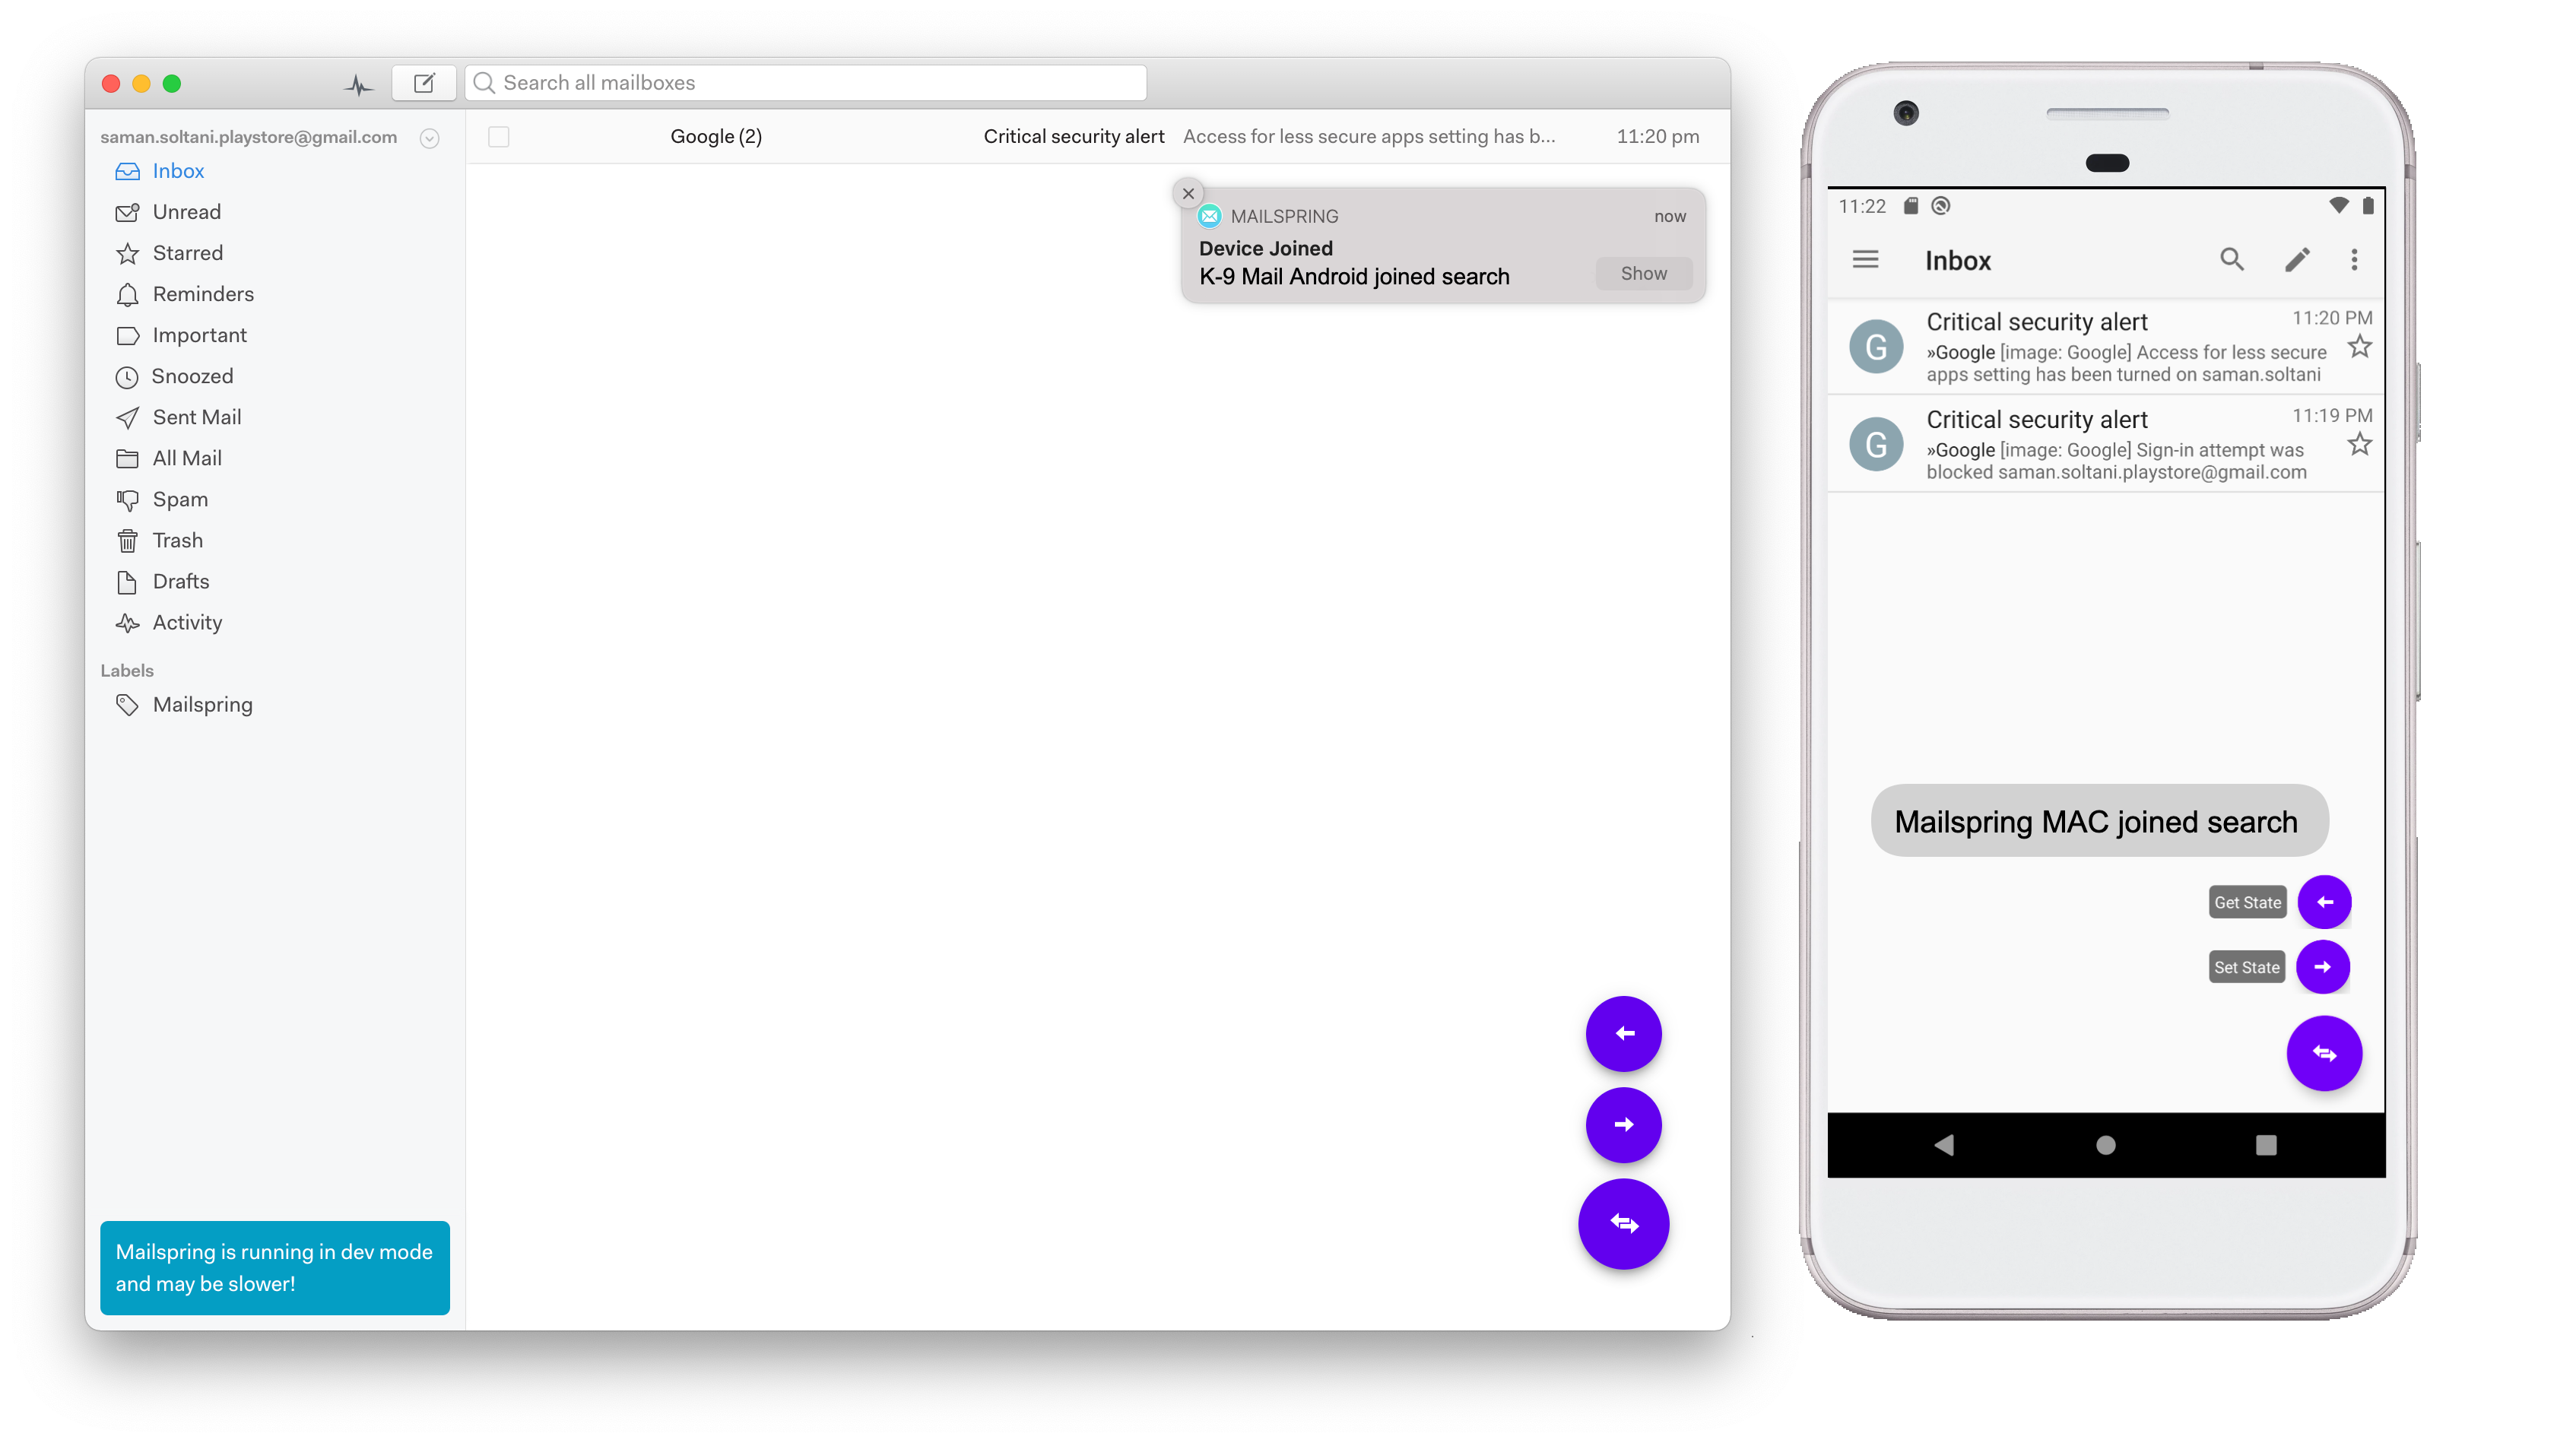
\includegraphics[width=\linewidth]{../figures/adapt-noti.png}
    \centering
    \caption{Screenshot of Native Notifications and Run-time State Migration Button}
    \label{fig:adapt-noti}
\end{figure}
\FloatBarrier

Figure \ref{fig:adapt-compose} shows the compose window of Mailspring and K-9 Mail which have a run-time state migration button.

\FloatBarrier
\begin{figure}[H]
    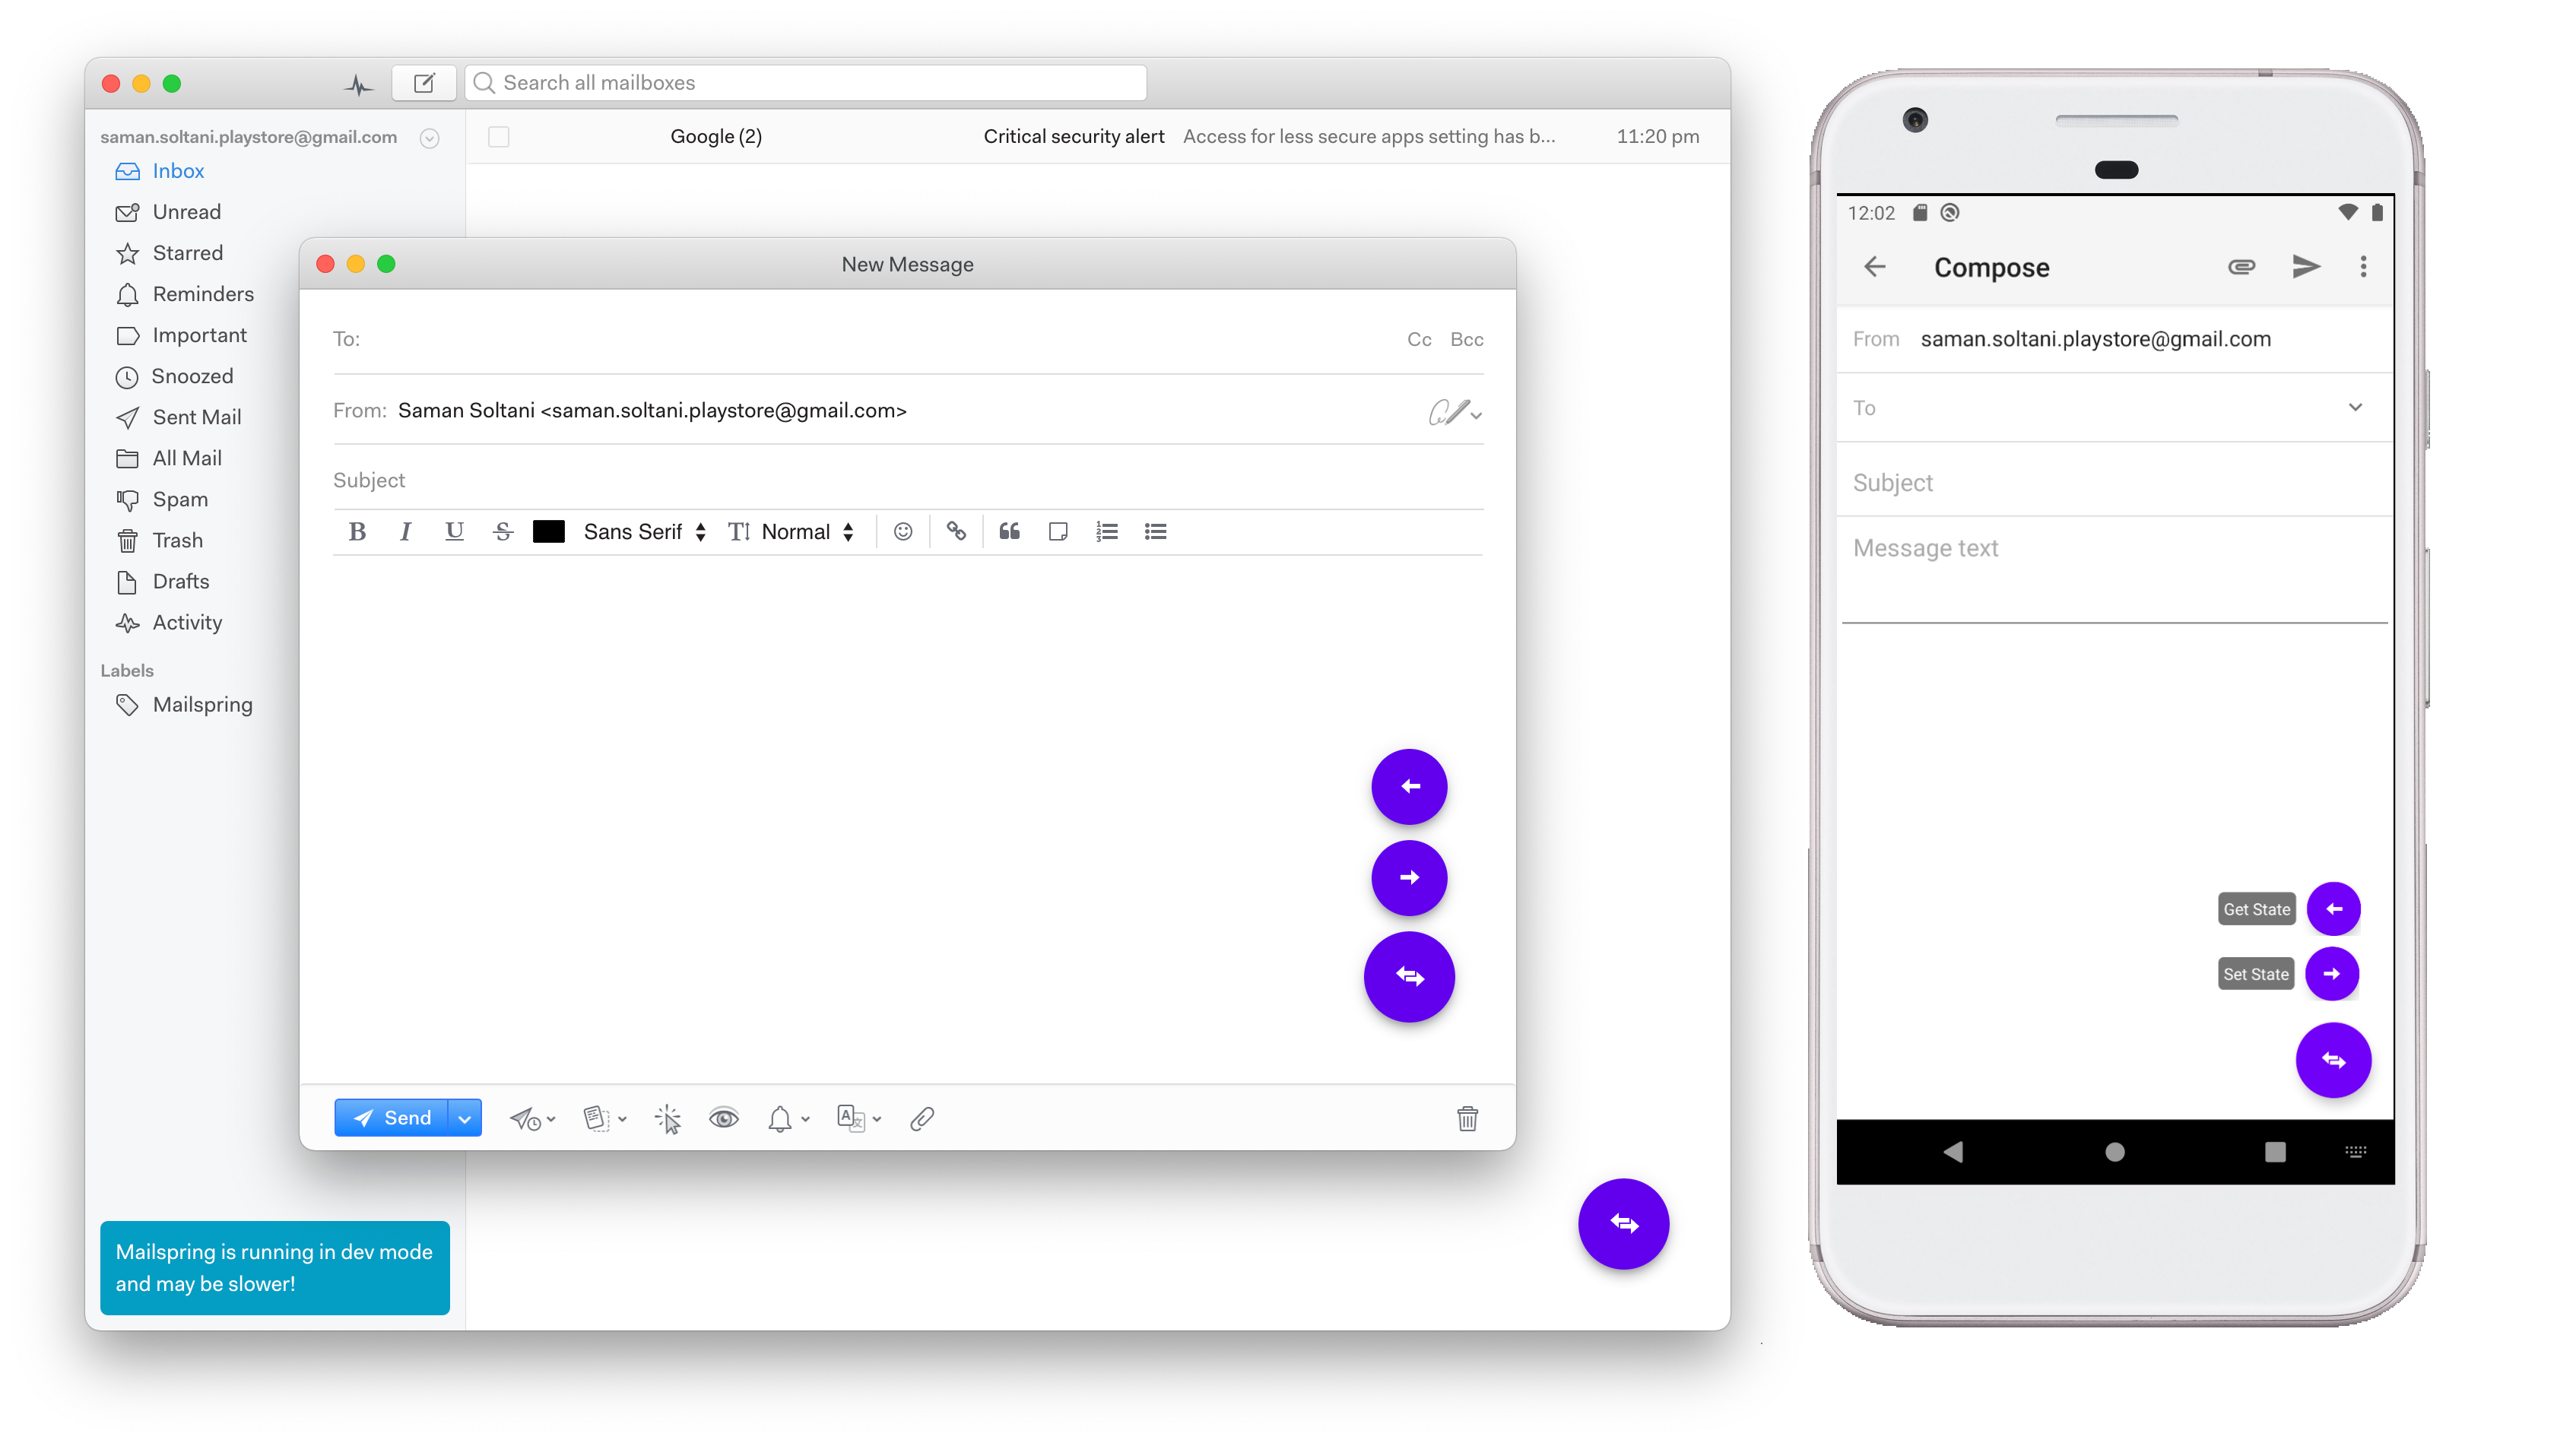
\includegraphics[width=\linewidth]{../figures/adapt-compose.png}
    \centering
    \caption{Screenshot of Compose Window}
    \label{fig:adapt-compose}
\end{figure}
\FloatBarrier

Figure \ref{fig:adapt-modal} shows the device modal of Mailspring and K-9 Mail which have a migrate button.

\FloatBarrier
\begin{figure}[H]
    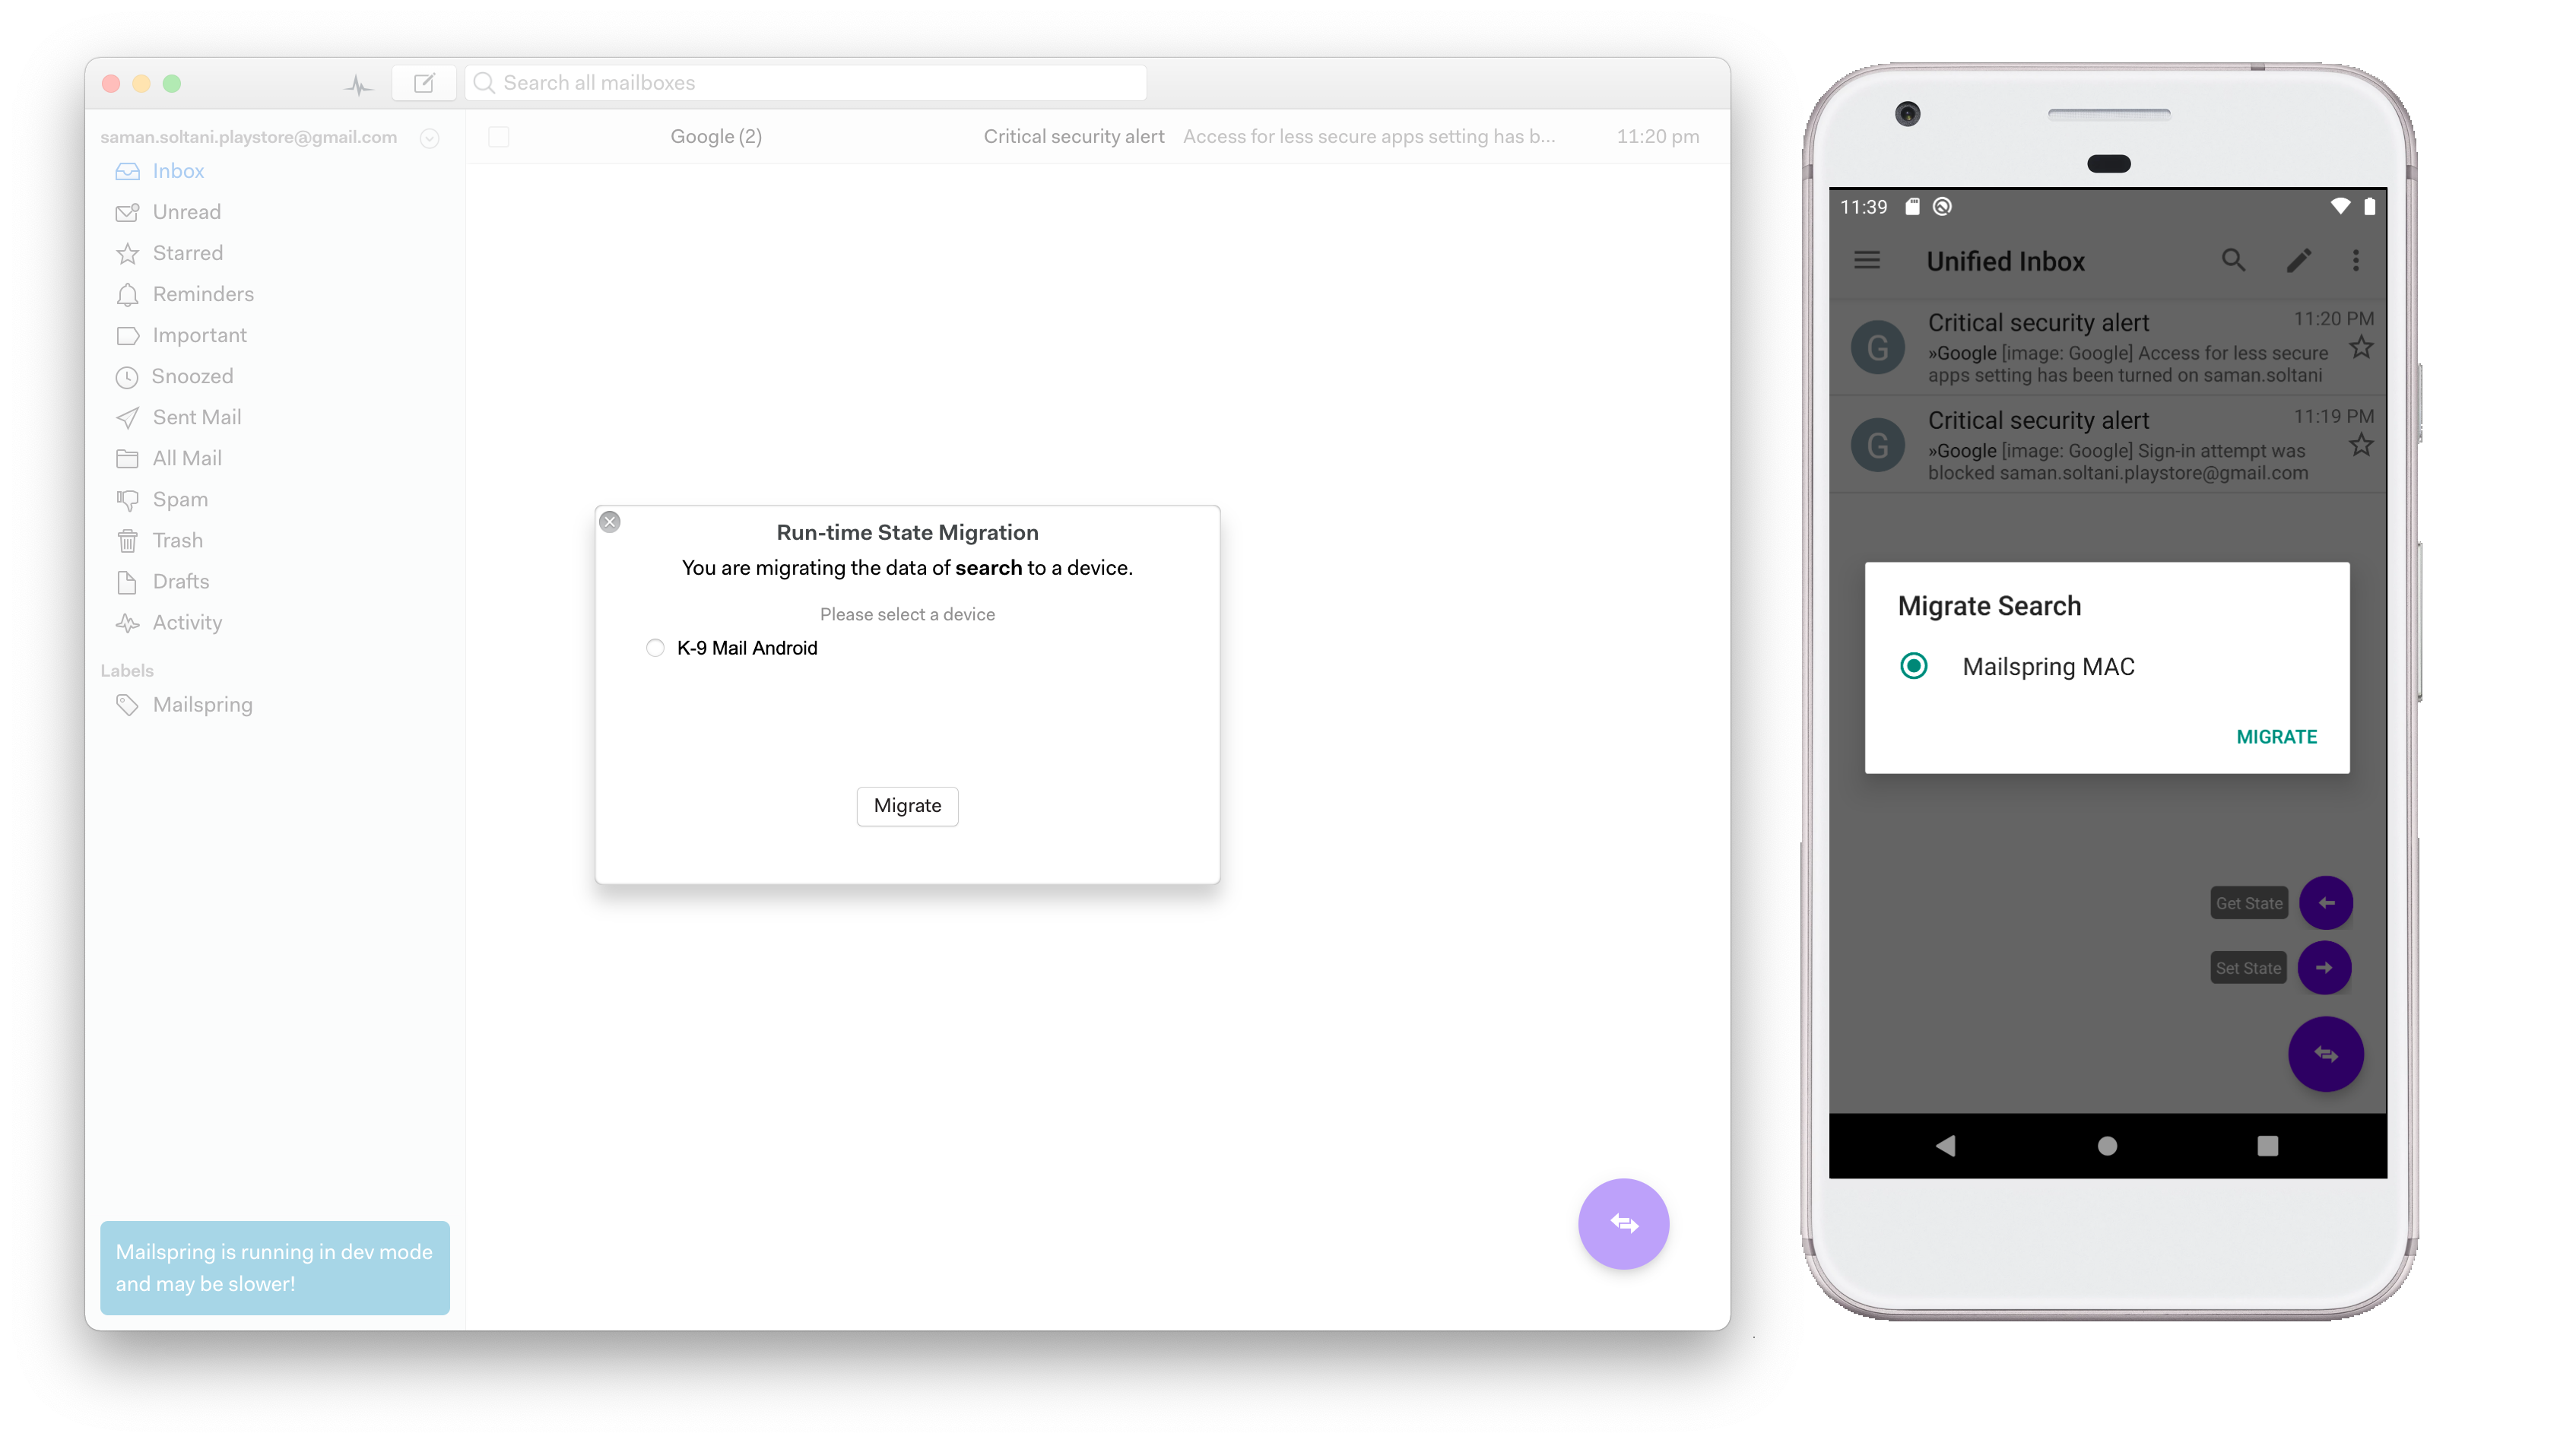
\includegraphics[width=\linewidth]{../figures/adapt-modal.png}
    \centering
    \caption{Screenshot of Device List Modal Box}
    \label{fig:adapt-modal}
\end{figure}
\FloatBarrier


